\documentclass[11pt,leqno]{article}

\usepackage[all]{xy}
%\usepackage{amsmath,amssymb}
%auto-ignore
%!TEX root = webs.tex
%this ensures the arxiv doesn't try to start TeXing here.

\usepackage{amsmath,amssymb,amsfonts,amsthm}
\usepackage{ifpdf}

\usepackage{comment}

\usepackage[all]{xy}
\SelectTips{cm}{}
% This may speed up compilation of complex documents with many xymatrices.
%\CompileMatrices

\usepackage[section]{placeins}
\usepackage{leftidx}
\usepackage{stmaryrd} % additional math symbols, e.g. \mapsfrom
%\usepackage{libertine}
%\usepackage[T1]{fontenc}
\usepackage{microtype}

% ----------------------------------------------------------------
\vfuzz5pt % Don't report over-full v-boxes if over-edge is small
\hfuzz5pt % Don't report over-full h-boxes if over-edge is small
% ----------------------------------------------------------------

% don't warn about PDF 1.5 (default was 1.4); dangerous?
\pdfminorversion=5

% diagrams -------------------------------------------------------
% figures ---------------------------------------------------------
\newcommand{\pathtotrunk}{./}
\newcommand{\pathtodiagrams}{\pathtotrunk}

\newcommand{\mathfig}[2]{\ensuremath{\hspace{-3pt}\begin{array}{c}%
  \raisebox{-2.5pt}{\includegraphics[width=#1\textwidth]{\pathtodiagrams #2}}%
\end{array}\hspace{-3pt}}}
\newcommand{\reflectmathfig}[2]{{\hspace{-3pt}\begin{array}{c}%
  \raisebox{-2.5pt}{\reflectbox{\includegraphics[width=#1\textwidth]{\pathtodiagrams #2}}}%
\end{array}\hspace{-3pt}}}
\newcommand{\rotatemathfig}[3]{{\hspace{-3pt}\begin{array}{c}%
  \raisebox{-2.5pt}{\rotatebox{#2}{\includegraphics[height=#1\textwidth]{\pathtodiagrams #3}}}%
\end{array}\hspace{-3pt}}}
\newcommand{\placefig}[2]{\includegraphics[width=#1\linewidth]{\pathtodiagrams #2}}

\newcommand{\arxiv}[1]{\href{http://arxiv.org/abs/#1}{\tt arXiv:\nolinkurl{#1}}}
\newcommand{\doi}[1]{\href{http://dx.doi.org/#1}{{\tt DOI:#1}}}
\newcommand{\euclid}[1]{\href{http://projecteuclid.org/euclid.cmp/#1}{{\tt #1}}}
\newcommand{\mathscinet}[1]{\href{http://www.ams.org/mathscinet-getitem?mr=#1}{\tt #1}}
\newcommand{\googlebooks}[1]{(preview at \href{http://books.google.com/books?id=#1}{google books})}


% THEOREMS -------------------------------------------------------
\theoremstyle{plain}
%\newtheorem*{fact}{Fact}
\newtheorem{prop}{Proposition}[subsection]
\makeatletter
\@addtoreset{prop}{section}
\makeatother
\newtheorem{conj}[prop]{Conjecture}
\newtheorem{thm}[prop]{Theorem}
\newtheorem{lem}[prop]{Lemma}
\newtheorem*{lem*}{Lemma}
\newtheorem{cor}[prop]{Corollary}
\newtheorem*{cor*}{Corollary}
\newtheorem*{exc}{Exercise}
\newtheorem{defn}[prop]{Definition}         % numbered definition
\newtheorem*{defn*}{Definition}             % unnumbered definition
\newtheorem{question}{Question}
\newtheorem{property}[prop]{Property}
\newenvironment{rem}{\vspace{0.3cm}\noindent\textsl{Remark.}}{}  % perhaps looks better than rem above?
\newenvironment{example}{\vspace{0.3cm}\noindent\textbf{Example.}}{}  % perhaps looks better than rem above?
\newtheorem{rem*}[prop]{Remark}
\numberwithin{equation}{section}
%% example, claim and remark are defined in article_preamble.tex, for compatibility with beamer and PNAS


% Marginal notes in draft mode -----------------------------------
\newcounter{comment}
\newcommand{\noop}[1]{}
\newcommand{\todo}[1]{\textbf{\color[rgb]{.8,.2,.5}\small TODO: #1}}

% \mathrlap -- a horizontal \smash--------------------------------
% For comparison, the existing overlap macros:
% \def\llap#1{\hbox to 0pt{\hss#1}}
% \def\rlap#1{\hbox to 0pt{#1\hss}}
\def\clap#1{\hbox to 0pt{\hss#1\hss}}
\def\mathllap{\mathpalette\mathllapinternal}
\def\mathrlap{\mathpalette\mathrlapinternal}
\def\mathclap{\mathpalette\mathclapinternal}
\def\mathllapinternal#1#2{%
\llap{$\mathsurround=0pt#1{#2}$}}
\def\mathrlapinternal#1#2{%
\rlap{$\mathsurround=0pt#1{#2}$}}
\def\mathclapinternal#1#2{%
\clap{$\mathsurround=0pt#1{#2}$}}

% MATH -----------------------------------------------------------
\newcommand{\id}{\boldsymbol{1}}
\renewcommand{\imath}{\mathfrak{i}}
\renewcommand{\jmath}{\mathfrak{j}}

\newcommand{\ssum}[1]{\Sigma#1}
\newcommand{\sumhat}{\overline{\sum}}
\newcommand{\sumtah}{\underline{\sum}}

\newcommand{\lmod}[1]{\leftidx{_{#1}}{\operatorname{mod}}{}}

\newcommand{\into}{\hookrightarrow}
\newcommand{\onto}{\twoheadrightarrow}
\newcommand{\iso}{\cong}
\newcommand{\quism}{\underset{\text{q.i.}}{\simeq}}
\newcommand{\htpy}{\simeq}
\newcommand{\actsOn}{\circlearrowright}
\newcommand{\xto}[1]{\xrightarrow{#1}}
\newcommand{\isoto}{\xto{\iso}}
\newcommand{\quismto}{\xrightarrow[\text{q.i.}]{\iso}}
\newcommand{\diffeoto}{\xrightarrow[\text{diffeo}]{\iso}}
\newcommand{\htpyto}{\xrightarrow[\text{htpy}]{\htpy}}

\newcommand{\restrict}[2]{#1{}_{\mid #2}{}}
\newcommand{\set}[1]{\left\{#1\right\}}
\newcommand{\setc}[2]{\setcl{#1}{#2}}
\newcommand{\setcl}[2]{\left\{ \left. #1 \;\right| \; #2 \right\}}
\newcommand{\setcr}[2]{\left\{ #1 \;\left| \; #2 \right\}\right.}

\newcommand{\floor}[1]{\left\lfloor#1\right\rfloor}
\newcommand{\norm}[1]{\left|\left|#1\right|\right|}
\newcommand{\abs}[1]{\left|#1\right|}

\newcommand{\qi}[2][q]{\left[#2\right]_{#1}}
\newcommand{\qBinomial}[3][q]{\genfrac{[}{]}{0pt}{}{#2}{#3}_{#1}}
\newcommand{\qPoch}[3]{\left(#1;#2\right)_{#3}}

\newcommand{\card}[1]{\sharp{#1}}

\newcommand{\bdy}{\partial}
\newcommand{\compose}{\circ}
\newcommand{\eset}{\emptyset}

\newcommand{\directSum}{\oplus}
\newcommand{\DirectSum}{\bigoplus}
\newcommand{\tensor}{\otimes}
\newcommand{\Tensor}{\bigotimes}

\newcommand{\Homa}[3]{\Hom_{#1}\left(#2,#3\right)}
\newcommand{\Hom}{\operatorname{Hom}}
\newcommand{\End}[1]{\operatorname{End}\left(#1\right)}

% ----------------------------------------------------------------

\ifpdf
	\usepackage[pdftex,plainpages=false,hypertexnames=false,pdfpagelabels]{hyperref}
	\usepackage[pdftex]{graphicx}
\else
	\usepackage[plainpages=false,hypertexnames=false,pdfpagelabels]{hyperref}
	\usepackage{graphicx}
\fi

%must load tikz after graphicx
\usepackage{tikz}
\usetikzlibrary{shapes}
\usetikzlibrary{backgrounds}
\usetikzlibrary{decorations,decorations.pathreplacing,decorations.markings}
\usetikzlibrary{fit,calc,through}
\usetikzlibrary{external}

\tikzstyle{mid>}=[decoration={markings, mark=at position 0.5 with {\arrow{>}}}, postaction={decorate}]
\tikzstyle{mid<}=[decoration={markings, mark=at position 0.5 with {\arrow{<}}}, postaction={decorate}]
\tikzstyle{upper>}=[decoration={markings, mark=at position 0.8 with {\arrow{>}}}, postaction={decorate}]
\tikzstyle{upper<}=[decoration={markings, mark=at position 0.8 with {\arrow{<}}}, postaction={decorate}]
\tikzstyle{lower>}=[decoration={markings, mark=at position 0.2 with {\arrow{>}}}, postaction={decorate}]
\tikzstyle{lower<}=[decoration={markings, mark=at position 0.2 with {\arrow{<}}}, postaction={decorate}]

\def\Foam{{\mathcal{F}{\rm oam}}}
\newcommand{\alt}{\wedge}
\newcommand{\Alt}[2]{{\textstyle\bigwedge^{#1}_{#2}}}
\newcommand{\Usl}[1]{U\sl_{#1}}
\newcommand{\one}{1}
\def\sA{\mathcal{A}}
\def\l{\lambda}
\def\bZ{{\mathbb{Z}}}
\def\sl{{\mathfrak{sl}}}
\def\Sp{{\mathcal{S}p}}
\def\FSp{{\mathcal{FS}p}}
\def\bC{{\mathbb{C}}}
\def\g{{\mathfrak{g}}}
\def\SL{{\rm{SL}}}
\def\GL{{\rm{GL}}}
\def\gl{{\mathfrak{gl}}}
\def\dU{\dot{{\mathcal{U}}}_q}
\def\Uq{\mathcal{U}_q}
\def\Rep{\mathcal{R}ep}
\def\la{\langle}
\def\ra{\rangle}
\def\dalg{\dot{{U}}_q}

\newcommand{\ul}[1]{{\underline{#1}}}

%\newcommand{\RepSL}[1]{\mathcal{R}ep(SL_{#1})}
\newcommand{\Lad}{\mathcal{L}ad}

\usepackage{environ}
\usepackage{xargs}

\newcommandx{\NewEnvironx}[5][2,3]{%
  \expandafter\newcommandx\csname start#1\endcsname[#2][#3]{#4}%
  \NewEnviron{#1}{\csname start#1\expandafter\endcsname\BODY #5}}

\newcommand{\ladderX}{1.5}
\newcommand{\ladderY}{1.5}
\newcommand{\ladderR}{0.6}
\newcommand{\laddercoordinates}[2]{
\foreach \x in {0,...,#1} {
	\foreach \y in {0,...,#2} {
		\coordinate (l\x\y) at (\x * \ladderX, \y * \ladderY);
		\coordinate (u\x\y) at ($(l\x\y)+\ladderR*(0,\ladderY)$);
		\coordinate (d\x\y) at ($(l\x\y)+(0,\ladderY)-\ladderR*(0,\ladderY)$);
	}
}
}
\newcommand{\ladderEn}[5]{
\draw[mid>] (l#1#2) -- (d#1#2);
\draw[mid>] (d#1#2) -- ($(l#1#2)+(0,\ladderY)$) node[left] {#3};
\draw[mid>] ($(l#1#2)+(\ladderX,0)$) -- ($(u#1#2)+(\ladderX,0)$);
\draw[mid>] ($(u#1#2)+(\ladderX,0)$) -- ($(l#1#2)+(\ladderX,\ladderY)$) node[right] {#4};
\draw[mid>] (d#1#2) --node[above]{#5} ($(u#1#2)+(\ladderX,0)$);
}
\newcommand{\ladderE}[4]{\ladderEn{#1}{#2}{#3}{#4}{}}
\newcommand{\ladderFn}[5]{
\draw[mid>] (l#1#2) -- (u#1#2);
\draw[mid>] (u#1#2) -- ($(l#1#2)+(0,\ladderY)$) node[left] {#3};
\draw[mid>] ($(l#1#2)+(\ladderX,0)$) -- ($(d#1#2)+(\ladderX,0)$);
\draw[mid>] ($(d#1#2)+(\ladderX,0)$) -- ($(l#1#2)+(\ladderX,\ladderY)$) node[right] {#4};
\draw[mid>] ($(d#1#2)+(\ladderX,0)$) --node[above]{#5} (u#1#2);
}
\newcommand{\ladderF}[4]{\ladderFn{#1}{#2}{#3}{#4}{}}
\newcommand{\ladderIn}[3]{\draw[mid>] (l#1#2) -- +($#3*(0,\ladderY)$);}
\newcommand{\ladderI}[2]{\ladderIn{#1}{#2}{1}}

\NewEnvironx{ladder}[2]{%
  \begin{tikzpicture}[baseline=13*\ladderY*#2]\laddercoordinates{#1}{#2}}
{\end{tikzpicture}}

\newcommand{\fuse}[3]{\tikz[baseline=0.5cm]{
\coordinate (z1) at (0,0);
\coordinate (z2) at (1,0);
\coordinate (c) at (0.5,0.5);
\coordinate (e) at (0.5,1);
\draw[mid>] (z1) node[below] {$#1$} -- (c);
\draw[mid>] (z2) node[below] {$#2$} -- (c);
\draw[mid>] (c) -- (e) node[above] {$#3$};
}}
\newcommand{\fork}[3]{\tikz[baseline=0.5cm]{
\coordinate (z1) at (0,1);
\coordinate (z2) at (1,1);
\coordinate (c) at (0.5,0.5);
\coordinate (e) at (0.5,0);
\draw[mid<] (z1) node[above] {$#1$} -- (c);
\draw[mid<] (z2) node[above] {$#2$} -- (c);
\draw[mid<] (c) -- (e) node[below] {$#3$};
}}


% example for creating tikz environments compatible with externalize
% thanks Andrew Stacey: http://tex.stackexchange.com/a/15614/77
%\NewEnvironx{mytikz}[1][1=]{%
%  \begin{figure}[htp]
%  \centering
%  \begin{tikzpicture}[#1]}
%{\end{tikzpicture}
%  \end{figure}}

% tricky way to iterate macros over a list
\def\semicolon{;}
\def\applytolist#1{
    \expandafter\def\csname multi#1\endcsname##1{
        \def\multiack{##1}\ifx\multiack\semicolon
            \def\next{\relax}
        \else
            \csname #1\endcsname{##1}
            \def\next{\csname multi#1\endcsname}
        \fi
        \next}
    \csname multi#1\endcsname}

% \def\cA{{\cal A}} for A..Z
\def\calc#1{\expandafter\def\csname c#1\endcsname{{\mathcal #1}}}
\applytolist{calc}QWERTYUIOPLKJHGFDSAZXCVBNM;

\usepackage{color}

% idea from tex-overflow
\usepackage{xcolor}
\definecolor{dark-red}{rgb}{0.7,0.25,0.25}
\definecolor{dark-blue}{rgb}{0.15,0.15,0.55}
\definecolor{medium-blue}{rgb}{0,0,0.65}
\hypersetup{
    colorlinks, linkcolor={dark-red},
    citecolor={dark-blue}, urlcolor={medium-blue}
}


% margin stuff
\setlength{\textwidth}{6.5in}
\setlength{\oddsidemargin}{0in}
\setlength{\evensidemargin}{0in}
\setlength{\textheight}{8.5in}
\setlength{\topmargin}{-.25in}



\title{something about webs and skew Howe duality}
\author{Sabin~Cautis, Joel~Kamnitzer and Scott~Morrison}

\begin{document}

\makeatletter
\@addtoreset{equation}{section}
\gdef\theequation{\thesection.\arabic{equation}}
\makeatother

\maketitle

\begin{abstract}
\end{abstract}

\hypersetup{
    colorlinks, linkcolor={black},
    citecolor={dark-blue}, urlcolor={medium-blue}
}

\tableofcontents

\hypersetup{
    colorlinks, linkcolor={dark-red},
    citecolor={dark-blue}, urlcolor={medium-blue}
}

\newcommand{\alt}{\wedge}

\newcommand{\Alt}{\bigwedge}

\renewcommand{\sl}[1]{\mathfrak{sl}_{#1}}
\newcommand{\Usl}[1]{U\sl{#1}}

\newcommand{\one}{1}

\newcommand{\gl}[1]{\mathfrak{gl}_{#1}}
\newcommand{\Ugl}[1]{U\gl{#1}}

\newcommand{\ul}[1]{{\underline{#1}}}

\newcommand{\RepSL}[1]{\mathcal{R}ep(SL_{#1})}
\newcommand{\Lad}{\mathcal{L}ad}

\section{Introduction}
The representation theory of $\sl{n}$ is a pivotal tensor category, and it is natural to ask for a presentation by generators and relations, as a pivotal tensor category.

There are two main choices one needs to make before looking for such a presentation. First, it would be reasonable to pass to any full subcategory, whose idempotent completion recovers the entire representation theory. In particular, in this paper we look at the full subcategory (denoted $\RepSL{n}$) whose objects are isomorphic to tensor products of the fundamental representations $\Alt^k \mathbb C^n$ of $\sl{n}$. (It might alternatively be interesting to descend all the way to the full subcategory whose objects are tensor powers of the standard representation.) Second, we need to decide which generators to use. We take the maps $\Alt^a \mathbb{C}^n \tensor \Alt^b \mathbb{C}^n \tensor \Alt^c \mathbb{C}^n \to \mathbb{C}$. (The space of such maps is one-dimensional if $a+b+c$ is a multiple of $n$, or zero-dimensional otherwise.) It is relatively easy to show that these are indeed generators, i.e. that every $\sl{n}$-linear map between tensor products of fundamental representations can be written as tensor products and compositions of these maps, along with the duality pairing and copairing maps \cite[Proposition 3.5.8]{0704.1503}. The question then, is to identify the relations holding between such planar compositions.

Said another way, we have a pivotal category of trivalent webs, with oriented edges labelled by $\{0, \ldots, n\}$, and at each vertex the labels summing to a multiple of $n$, and a full and dominant functor to the representation theory category. The question is to identify the pivotal ideal which is the kernel of this functor.

This problem has been studied previously. For $n=2$, there are no trivalent vertices, and the category of webs is essentially just the category of embedded 1-manifolds up to isotopy. The kernel of the functor to representation theory is the ideal generated by the difference $\tikz[baseline=-2pt]{\node[draw,circle] {};} - 2$. \todo{Explain that this is Temperley-Lieb.}

For $n=3$ .... \todo{talk about Kuperberg's relations for $\sl{3}$ \cite{MR1403861}.}

For $n \geq 4$, generators for the kernel have been proposed, by \cite{math.QA/0310143} (for $n=4$) and by \cite{0704.1503} (generally), but without proving that their lists of relations were complete.

This paper answers the question, in particular showing that the relations of \cite{0704.1503} are complete. In fact, those relations were unnecessarily complete; just the $I=H$ and `square-switch' relations suffice, and generate the others. The relevant relations are reproduced in \S\ref{sec:diagrams}.
The main theorem, stating the isomorphism between a combinatorially defined web category and the representation theory of $\Usl{n}$, appears in \S \ref{sec:theorem}.

The core idea of our proof is to use skew Howe duality (see \S \ref{sec:skew-howe}). In fact we give a very succinct recipe for the relations, as certain truncations of relations holding in $\Usl{m}$. We now give a quick overview of the argument.

We denote the quotient of the category of trivalent webs by the $I=H$ and square switch relations as $Sp(SL_n)$. We have a surjective functor to the the representation theory, which we would like to show is an isomorphism. All that remains is to check that it is injective on morphisms.

Skew Howe duality states that the commuting actions of $\Usl{n}$ and $\Usl{m}$ on $\Alt^\bullet(\mathbb{C}^n \tensor \mathbb{C}^m)$ are in fact each the commutant of the other. That is, if  $f: \Alt^\bullet(\mathbb{C}^n \tensor \mathbb{C}^m) \to \Alt^\bullet(\mathbb{C}^n \tensor \mathbb{C}^m)$ is $\sl{n}$-linear, then there is some element $X_f \in \Usl{m}$ whose action on  $\Alt^\bullet(\mathbb{C}^n \tensor \mathbb{C}^m)$ is exactly $f$.

Suppose we have some element $A \in \Homa{Sp(SL_n)}{\underline{k}}{\underline{k'}}$ which maps to zero in the representation theory. (Here $\underline{k}$ and $\underline{k}$ denote two sequences of integers in $\{0,\ldots,n\}$, i.e. two objects in $Sp(SL_n)$.) We would like to show that $A$ is itself zero. We first define a related element $\tilde{A} \in \Homa{Sp(SL_n)}{\underline{l}}{\underline{l'}}$, where $\underline{l}$ is obtained from $\underline{k}$ by interposing some number of $0$s and $n$s, and similarly for $\underline{l'}$, and further $\underline{l}$ and $\underline{l'}$ have the same length $m$ and the same sum $L$. (Previously, the sums of $\underline{k}$ and $\underline{k'}$ might be differed by a multiple of $n$.) This element $\tilde{A}$ is a linear combination of `ladder diagrams', those web diagrams of the following form:
\todo{an example ladder diagram}
A complete description of ladder diagrams and the construction of $\tilde{A}$ from $A$ appears in \S \ref{sec:ladders}.

Now, rewriting $\Alt^L(\mathbb C^n \tensor \mathbb C^m)$ as
\begin{align*}
\alt^L(\mathbb C^n \tensor \mathbb C^m) & = \alt^L(\mathbb C^n \directSum \cdots \directSum \mathbb C^n) \\
        & = \DirectSum_{\underline{l}: \sum \underline{l} = L} \alt^{l_1} \mathbb C^n \tensor \cdots \tensor \alt^{l_m} \mathbb C^n
\end{align*}
we see the objects $\underline{l}$ and $\underline{l}'$ as summands, and hence $\tilde{A}$ as an endomorphism of $\Alt^\bullet(\mathbb C^n \tensor \mathbb C^m)$. Thus there is some element $X_{\tilde{A}} \in \Usl{m}$, which acts by zero on $\Alt^\bullet(\mathbb C^n \tensor \mathbb C^m)$. In fact, since $\tilde{A}$ was a ladder diagram, we can write down an explicit element $X_{\tilde{A}}$, by interpreting each rung of the ladder as some $E^{(a)}_j$ or $F^{(a)}_j$ in $\Usl{m}$. 

Next, we find that we can explicitly describe the kernel of $\Usl{m}$ acting on $\Alt^\bullet(\mathbb C^n \tensor \mathbb C^m)$. The kernel is precisely the ideal generated by those weight space idempotents falling outside the weight support of $\Alt^\bullet(\mathbb C^n \tensor \mathbb C^m)$. \todo{Saying this requires having previously mentioned the idempotented form.} This result is proved in \S \ref{sec:kernel}.


\section{Web diagrams and relations}
\label{sec:diagrams}
\tikzstyle{mid>}=[decoration={markings, mark=at position 0.5 with {\arrow{>}}}, postaction={decorate}]
\tikzstyle{mid<}=[decoration={markings, mark=at position 0.5 with {\arrow{<}}}, postaction={decorate}]

The free spider category $FSp(SL_n)$ has as objects sequences $\ul{k}$ in $\{0^\pm,\ldots,n^\pm\}$, and as morphisms (linear combinations of) oriented planar graphs locally modeled on the following four types of vertices:
\newcommand{\fuse}[3]{\tikz[baseline=0.5cm]{
\coordinate (z1) at (0,0);
\coordinate (z2) at (1,0);
\coordinate (c) at (0.5,0.5);
\coordinate (e) at (0.5,1);
\draw[mid>] (z1) node[below] {$#1$} -- (c);
\draw[mid>] (z2) node[below] {$#2$} -- (c);
\draw[mid>] (c) -- (e) node[above] {$#3$};
}}
\newcommand{\fork}[3]{\tikz[baseline=0.5cm]{
\coordinate (z1) at (0,1);
\coordinate (z2) at (1,1);
\coordinate (c) at (0.5,0.5);
\coordinate (e) at (0.5,0);
\draw[mid<] (z1) node[above] {$#1$} -- (c);
\draw[mid<] (z2) node[above] {$#2$} -- (c);
\draw[mid<] (c) -- (e) node[below] {$#3$};
}}


\begin{align*}
\fuse{a}{b}{a+b}
\qquad
\fork{a}{b}{a+b}
\qquad
\tikz[baseline=0.7cm]{
\foreach \n in {0,1,2} {
	\coordinate (a\n) at (0.4*\n, 0.8*\n);
}
\draw[mid>] (a0) -- node[right] {$a$} (a1);
\draw[mid<] (a1) -- node[right] {$n-a$} (a2);
\draw (a1) -- +(-0.2,0.1);
}
\qquad
\tikz[baseline=0.7cm]{
\foreach \n in {0,1,2} {
	\coordinate (a\n) at (0.4*\n, 0.8*\n);
}
\draw[mid<] (a0) -- node[right] {$a$} (a1);
\draw[mid>] (a1) -- node[right] {$n-a$} (a2);
\draw (a1) -- +(-0.2,0.1);
}
\end{align*}
with all labels drawn from the set $\{1,\ldots,n-1\}$.
(The third and fourth are bivalent vertices, called `tags', which are not rotationally symmetric; the tag provides a distinguished side.) The source and target of a morphism determine the labels which must appear around the boundary. The bottom boundary of the planar graph in $\Hom(\ul{k}, \ul{k'})$ must have boundary agreeing with the source object $\ul{k}$, ignoring any $0^\pm$ or $n^\pm$ entries, and with the strand oriented up for each positive entry, and the strand oriented down for each negative entry. Similary, the top boundary is determined from $\ul{k'}$ in the same way.
\begin{example}
\todo{some examples}
\end{example}
Note that any given graph lies in many distinct $\Hom$ spaces: we can always insert additional $0^\pm$ and $n^\pm$ in the source or target. In fact, whenever we add or remove a $0^\pm$ or $n^\pm$ in a sequence $\ul{k}$, we obtain an isomorphic object (just take the identity diagram: the appropriately oriented vertical strings labelled by the other elements of $\ul{k}$). We could skeletonize the category by throwing out all these redundant objects, but it's more convenient to keep them.

We will often draw diagrams with edges also labelled by $0$ or $n$. This is a notational convenience, to be interpreted as follows. Edges labelled by $0$ and $n$ are to be deleted; trivalent vertices involving a $0$ edge become simple strands, and trivalent vertices involving a $n$ edge are replaced by tags:
\begin{align*}
\fuse{a}{n-a}{n} & = \tikz[baseline=0.5cm]{\draw[mid>] (0,0) node[below] {$a$} arc (180:90:0.6) node[coordinate] (c) {}; \draw[mid<] (c) arc (90:0:0.6) node[below] {$n-a$}; \draw (c) -- +(0,0.2);} &
\fork{a}{n-a}{n} & = \tikz[baseline=-0.5cm]{\draw[mid<] (0,0) node[above] {$a$} arc (-180:-90:0.6) node[coordinate] (c) {}; \draw[mid>] (c) arc (-90:0:0.6) node[above] {$n-a$}; \draw (c) -- +(0,0.2);} 
\end{align*}
(Any trivalent vertices with all edges labelled either $0$ or $n$ can simply be deleted.) In fact, we'll sometimes draw diagrams with edges less than $0$ or greater than $n$, and these are simply zero.

The spider category $Sp(SL_n)$ is the quotient of $FSp(SL_n)$ by the following relations


\newcommand{\ladderX}{1.5}
\newcommand{\ladderY}{1.5}
\newcommand{\ladderR}{0.6}
\newcommand{\laddercoordinates}[2]{
\foreach \x in {0,...,#1} {
	\foreach \y in {0,...,#2} {
		\coordinate (l\x\y) at (\x * \ladderX, \y * \ladderY);
		\coordinate (u\x\y) at ($(l\x\y)+\ladderR*(0,\ladderY)$);
		\coordinate (d\x\y) at ($(l\x\y)+(0,\ladderY)-\ladderR*(0,\ladderY)$);
	}
}
}
\newcommand{\ladderEn}[5]{
\draw[mid>] (l#1#2) -- (d#1#2);
\draw[mid>] (d#1#2) -- ($(l#1#2)+(0,\ladderY)$) node[left] {#3};
\draw[mid>] ($(l#1#2)+(\ladderX,0)$) -- ($(u#1#2)+(\ladderX,0)$);
\draw[mid>] ($(u#1#2)+(\ladderX,0)$) -- ($(l#1#2)+(\ladderX,\ladderY)$) node[right] {#4};
\draw[mid>] (d#1#2) --node[above]{#5} ($(u#1#2)+(\ladderX,0)$);
}
\newcommand{\ladderE}[4]{\ladderEn{#1}{#2}{#3}{#4}{}}
\newcommand{\ladderFn}[5]{
\draw[mid>] (l#1#2) -- (u#1#2);
\draw[mid>] (u#1#2) -- ($(l#1#2)+(0,\ladderY)$) node[left] {#3};
\draw[mid>] ($(l#1#2)+(\ladderX,0)$) -- ($(d#1#2)+(\ladderX,0)$);
\draw[mid>] ($(d#1#2)+(\ladderX,0)$) -- ($(l#1#2)+(\ladderX,\ladderY)$) node[right] {#4};
\draw[mid>] ($(d#1#2)+(\ladderX,0)$) --node[above]{#5} (u#1#2);
}
\newcommand{\ladderF}[4]{\ladderFn{#1}{#2}{#3}{#4}{}}
\newcommand{\ladderIn}[3]{\draw[mid>] (l#1#2) -- +($#3*(0,\ladderY)$);}
\newcommand{\ladderI}[2]{\ladderIn{#1}{#2}{1}}
\newenvironment{ladder}[2]{%
\begin{tikzpicture}[baseline=13*\ladderY*#2]
\laddercoordinates{#1}{#2}
}%
{
\end{tikzpicture}
}

\begin{align}
\tikz[baseline=0.4cm]{
\foreach \n in {0,1,2} {
	\coordinate (a\n) at (0.4*\n, 0.8*\n);
}
\draw[mid>] (a0) -- node[right] {$a$} (a1);
\draw[mid<] (a1) -- node[right] {$n-a$} (a2);
\draw (a1) -- +(-0.2,0.1);
} 
& = (-1)^{(n+1)a}
\tikz[baseline=0.4cm]{
\foreach \n in {0,1,2} {
	\coordinate (a\n) at (0.4*\n, 0.8*\n);
}
\draw[mid>] (a0) -- node[right] {$a$} (a1);
\draw[mid<] (a1) -- node[right] {$n-a$} (a2);
\draw (a1) -- +(0.2,-0.1);
}
\displaybreak[1]
\label{eq:switch}
\\
\begin{tikzpicture}[baseline=20]
\foreach \n in {0,...,3} {
	\coordinate (z\n) at (0.4*\n, 0.8*\n);
}
\draw[mid>] (z0) -- node[right] {$a+b$} (z1);
\draw[mid>] (z2) -- node[right] {$a+b$} (z3);
\draw[mid>] (z1) to[out=150,in=-190] node[left] {$a$} (z2);
\draw[mid>] (z1) to[out=-30,in=0] node[right] {$b$} (z2);
\end{tikzpicture}
& = \qBinomial{a+b}{a}
\tikz[baseline=20]{\draw[mid>] (0,0) -- node[right] {$a+b$} (1,2);}
\label{eq:bigon1}
\displaybreak[1] \\
\begin{tikzpicture}[baseline=20]
\foreach \n in {0,...,3} {
	\coordinate (z\n) at (0.4*\n, 0.8*\n);
}
\draw[mid>] (z0) -- node[right] {$a$} (z1);
\draw[mid>] (z2) -- node[right] {$a$} (z3);
\draw[mid<] (z1) to[out=150,in=-190] node[left] {$b$} (z2);
\draw[mid>] (z1) to[out=-30,in=0] node[right] {$a+b$} (z2);
\end{tikzpicture}
& = \qBinomial{n-a}{b}
\tikz[baseline=20]{\draw[mid>] (0,0) -- node[right] {$a$} (1,2);}
\label{eq:bigon2}
\displaybreak[1] \\
\begin{tikzpicture}[baseline]
\foreach \x/\y in {0/0,1/0,2/0,0/1,1/1,0/2} {
	\coordinate(z\x\y) at (\x+\y/2,\y/1.5);
}
\coordinate (z03) at (1,2);
\draw[mid>] (z00) node[below] {$a$} --  (z01);
\draw[mid>] (z01) -- node[left] {$a+b$} (z02);
\draw[mid>] (z10) node[below] {$b$} -- (z01);
\draw[mid>] (z20) node[below] {$c$} -- (z02); 
\draw[mid>](z02) -- node[left] {$a+b+c$} (z03);
\end{tikzpicture}
& =
\begin{tikzpicture}[baseline]
\foreach \x/\y in {0/0,1/0,2/0,0/1,1/1,0/2} {
	\coordinate(z\x\y) at (\x+\y/2,\y/1.5);
}
\coordinate (z03) at (1,2);
\draw[mid>] (z00) node[below] {$a$} --  (z02);
\draw[mid>] (z10) node[below] {$b$} -- (z11);
\draw[mid>] (z20) node[below] {$c$} -- (z11); 
\draw[mid>] (z11) -- node[right] {$b+c$} (z02);
\draw[mid>](z02) -- node[left] {$a+b+c$} (z03);
\end{tikzpicture}
\label{eq:IH}
\displaybreak[1] \\
\begin{tikzpicture}[baseline=40]
\laddercoordinates{1}{2}
\node[left] at (l00) {$a$};
\node[right] at (l10) {$b$};
\ladderEn{0}{0}{$a{-}1$}{$b{+}1$}{1}
\ladderFn{0}{1}{$a$}{$b$}{1}
\end{tikzpicture}
& =
\begin{tikzpicture}[baseline=40]
\laddercoordinates{1}{2}
\node[left] at (l00) {$a$};
\node[right] at (l10) {$b$};
\ladderFn{0}{0}{$a{+}1$}{$b{-}1$}{1}
\ladderEn{0}{1}{$a$}{$b$}{1}
\end{tikzpicture}
+
\qi{b-a}
\begin{tikzpicture}[baseline=40]
\laddercoordinates{1}{2}
\ladderIn{0}{0}{2}
\ladderIn{1}{0}{2}
\node[left] at (l02) {$a$};
\node[right] at (l12) {$b$};
\end{tikzpicture}
\label{eq:commutation}
\end{align}
\todo{We also need mirror reflections and the arrow reversals of these.}

Throughout below we'll refer to these as `switching a tag' (Relation \eqref{eq:switch}), `removing a bigon' (Relations \eqref{eq:bigon1, eq:bigon2}), `$I=H$' (Relation \eqref{eq:IH}) and `commutation' (Relation \eqref{eq:commutation}).

We'll also record several consequences of these relations, to be used later.
\begin{lem}
\begin{equation}
\tikz[baseline]{\draw[->] (0,0.5) node[above] {$a$} arc (45:-315:0.5cm);}  = \qBinomial{n}{a} \label{eq:loop}
\end{equation}
\end{lem}
\begin{proof}
This is just Relation \eqref{eq:bigon2} with $a=0$ after deleting the 0-strings.
\end{proof}
\begin{lem}
\begin{equation}
\tikz[baseline=0.6cm]{
\foreach \n in {0,1,2,3} {
	\coordinate (a\n) at (0.4*\n, 0.8*\n);
}
\draw[mid>] (a0) -- node[right] {$a$} (a1);
\draw[mid<] (a1) -- node[right] {$n-a$} (a2);
\draw[mid>] (a2) -- node[right] {$a$} (a3);
\draw (a1) -- +(-0.2,0.1);
\draw (a2) -- +(0.2,-0.1);
}  = \tikz[baseline=0.6cm]{\draw[mid>] (0,0) -- node[right] {$a$} (1.2,2.4);}
\end{equation}
\end{lem}
\begin{proof}
This is just the second bigon relation (Relation \eqref{eq:bigon2}) with $b=n-a$ after replacing the $n$-strand with a matching pair of tags. 
\end{proof}


\begin{lem}
\begin{equation}
\tikz[baseline=40]{
\laddercoordinates{1}{2}
\ladderEn{0}{0}{$a-s$}{$b+s$}{$s$}
\ladderEn{0}{1}{$a-s-r$}{$b+s+r$}{$r$}
\node[left] at (l00) {$a$};
\node[right] at (l10) {$b$};
}
=
\qBinomial{r+s}{r}
\tikz[baseline=20]{
\laddercoordinates{1}{1}
\ladderEn{0}{0}{$a-s-r$}{$b+s+r$}{$r+s$}
\node[left] at (l00) {$a$};
\node[right] at (l10) {$b$};
}
\end{equation}
\end{lem}
\begin{proof}
Use the $I=H$ relation twice, then remove a bigon.
\end{proof}

\begin{lem}
\begin{align}
\label{eq:commutation2}
\begin{ladder}{1}{2}
\node[left] at (l00) {$a$};
\node[right] at (l10) {$b$};
\ladderFn{0}{0}{$a+s$}{$b-s$}{$s$}
\ladderEn{0}{1}{$a+s-r$}{$b-s+r$}{$r$}
\end{ladder}
& = 
\sum_t (-1)^t \qBinomial{t+s-r-1+a-b}{t}
\begin{ladder}{1}{2}
\node[left] at (l00) {$a$};
\node[right] at (l10) {$b$};
\ladderEn{0}{0}{$a-r+t$}{$b+r-t$}{$r-t$}
\ladderFn{0}{1}{$a+s-r$}{$b-s+r$}{$s-t$}
\end{ladder}
\end{align}
\end{lem}
\begin{rem}
The summation over $t$ in Equation \eqref{eq:commutation2} is over the range $\max(b+r-n,r-a,0) \leq t \leq \min(s,r)$. If $t > s$ or $t>r$, the diagram vanishes (by convention) because there are labels less than zero. If $t<b+r-n$ the label on the right side of the square is greater than $n$. If $t<r-a$ the label on the left side is greater than $n$. If $t<0$ the quantum binomial vanishes. One may check that in each of the other terms all the labels are in $\{0,\ldots,n\}$.
\end{rem}
\begin{proof}
\todo{}
\end{proof}

{
In the next lemma, we begin using the convenient notation that any non-vertical strand which is not labelled implicitly carries a $1$, while unlabelled vertical strands are labelled arbitrarily.

\renewcommand{\ladderY}{1}
\begin{lem}
\begin{equation}
\begin{ladder}{2}{3}
\ladderE{0}{0}{}{}
\ladderE{0}{1}{}{}
\ladderE{1}{2}{}{}
\ladderI{0}{2}
\ladderIn{2}{0}{2}
\node[below] at (l00) {$a$};
\node[below] at (l10) {$b$};
\node[below] at (l20) {$c$};
\end{ladder}
- \qi{2}
\begin{ladder}{2}{3}
\ladderE{0}{0}{}{}
\ladderE{1}{1}{}{}
\ladderE{0}{2}{}{}
\ladderI{0}{1}
\ladderI{2}{0}
\ladderI{2}{2}
\end{ladder}
+
\begin{ladder}{2}{3}
\ladderE{1}{0}{}{}
\ladderE{0}{1}{}{}
\ladderE{0}{2}{}{}
\ladderI{0}{0}
\ladderIn{2}{1}{2}
\end{ladder}
= 0
\end{equation}
\end{lem}
\begin{proof}
In the middle term, apply the $I=H$ relation, obtaining
\begin{align*}
\begin{ladder}{2}{3}
\ladderE{0}{0}{}{}
\ladderE{1}{1}{}{}
\ladderE{0}{2}{}{}
\ladderI{0}{1}
\ladderI{2}{0}
\ladderI{2}{2}
\end{ladder}
& = 
\begin{tikzpicture}[baseline=40]
\laddercoordinates{2}{3}
\coordinate (m0) at ($(l00)!.5!(l03)$);
\coordinate (m2) at ($(l20)!.5!(l23)$);
\coordinate (m1m) at ($(m0)!.3!(m2)$);
\coordinate (m1p) at ($(m0)!.7!(m2)$);
\coordinate (m1d) at ($(l10)!.3!(l13)$);
\coordinate (m1u) at ($(l10)!.7!(l13)$);
\draw[mid>] (l00) -- (m0);
\draw[mid>] (m0) -- (l03);
\draw[mid>] (l20) -- (m2);
\draw[mid>] (m2) -- (l23);
\draw[mid>] (l10) -- (m1d);
\draw[mid>] (m1u) -- (l13);
\draw[mid>] (m0) -- node[above] {2} (m1m);
\draw[mid>] (m1p) -- (m2);
\draw[mid>] (m1m) -- (m1u);
\draw[mid>] (m1m) -- (m1d);
\draw[mid>] (m1d) --node[below right] {$b{+}1$} (m1p);
\draw[mid>] (m1p) --node[above right] {$b$} (m1u);
\end{tikzpicture} \\
\intertext{and now apply Equation \eqref{eq:commutation2} to the central square}
& = 
(-1)^0 ???
\begin{tikzpicture}[baseline=40]
\laddercoordinates{2}{3}
\coordinate (m0) at ($(l00)!.5!(l03)$);
\coordinate (m2) at ($(l20)!.5!(l23)$);
\coordinate (m1m) at ($(m0)!.3!(m2)$);
\coordinate (m1p) at ($(m0)!.7!(m2)$);
\coordinate (m1d) at ($(l10)!.3!(l13)$);
\coordinate (m1u) at ($(l10)!.7!(l13)$);
\draw[mid>] (l00) -- (m0);
\draw[mid>] (m0) -- (l03);
\draw[mid>] (l20) -- (m2);
\draw[mid>] (m2) -- (l23);
\draw[mid>] (l10) -- (m1d);
\draw[mid>] (m1u) -- (l13);
\draw[mid>] (m0) -- node[below] {2} (m1m);
\draw[mid>] (m1p) -- (m2);
\draw[mid>] (m1m) --node[above left] {$b+2$} (m1u);
\draw[mid<] (m1m) --node[below left] {$b$} (m1d);
\draw[mid<] (m1p) -- (m1u);
\end{tikzpicture}
+
(-1)^1 ???
\begin{tikzpicture}[baseline=40]
\laddercoordinates{2}{3}
\coordinate (m0) at ($(l00)!.5!(l03)$);
\coordinate (m2) at ($(l20)!.5!(l23)$);
\coordinate (m1m) at ($(m0)!.3!(m2)$);
\coordinate (m1p) at ($(m0)!.7!(m2)$);
\coordinate (m1d) at ($(l10)!.3!(l13)$);
\coordinate (m1u) at ($(l10)!.7!(l13)$);
\draw[mid>] (l00) -- (m0);
\draw[mid>] (m0) -- (l03);
\draw[mid>] (l20) -- (m2);
\draw[mid>] (m2) -- (l23);
\draw[mid>] (l10) -- (m1d);
\draw[mid>] (m1u) -- (l13);
\draw[mid>] (m0) -- node[above] {2} (m1m);
\draw[mid>] (m1p) -- (m2);
\draw[mid>] (m1m) --(m1u);
\draw[mid>] (m1d) --node[below right] {$b$} (m1p);
\draw[mid>] (m1p) --node[above right] {$b{-}1$} (m1u);
\end{tikzpicture}
\end{align*}
after which an application of the $I=H$ relation on each $2$-strand gives the desired identity.
\end{proof}
}


\begin{rem}
Just as a check:
Taking the `partial trace' of Relation \eqref{eq:commutation} (that is, closing up the $b$ endpoints), and evaluating all terms to a multiple of the $a$ strand using Relations \eqref{eq:bigon1} and \eqref{eq:bigon2}, we get the identity $\qBinomial{n-1}{b-1} \qi{n-a} = \qBinomial{n-1}{b} \qi{a} + \qBinomial{n}{b} \qi{b-a}$, which does in fact hold!
\end{rem}

\section{Skew Howe Duality}
\label{sec:skew-howe}

\subsection{The idempotent form of $ \Ugl{m} $}
\label{sec:idemform}
We now introduce the idempotent form of $\Ugl{m}$.  This is an algebra with generators $ E_i, F_i, \one_\ul{k} $, where $ \ul{k} = (k_1, \dots, k_m) \in \mathbb Z^m $.

It will be convenient for us to think of a $\Ugl{m} $ as a $\mathbb C$-linear category (which we will continue to denote $\Ugl{m}$) with objects $ \ul{k} $ and $ \Hom(\ul{k}, \ul{k'}) = \one_\ul{k} \Ugl{m} \one_\ul{k'}$.

Note that $ \Hom(\ul{k}, \ul{k'}) = 0 $ unless $ \sum k_i = \sum k'_i $.

\todo{More detail here.}

\subsection{The functor $F_m^n$}
Let $K $ be a positive integer.  The vector space $ \Alt^K(\mathbb C^n \otimes \mathbb C^m) $ carries commuting actions of both $ GL_m $ and $ GL_n $ and these actions generate each others commutant.  

Let us consider the weight decomposition of $\Alt^K(\mathbb C^n \otimes \mathbb C^m)$  with respect to the maximal torus of $ GL_m $.  It is given by 
\begin{equation}
 \Alt^K(\mathbb C^n \otimes \mathbb C^m) = \bigoplus_{\ul{k}} \alt^{k_1} \mathbb C^n \otimes \cdots \otimes \alt^{k_m} \mathbb C^n
 \end{equation}
where the sum ranges over those $ \ul{k} $ with $ 0 \le k_i \le n $ for all $ i $, and with $\sum \ul{k} = K$.  We will refer to these as the $n$-bounded weights of $ GL_m$.

As we have a $ GL_m$ action with these weight spaces, for any two $n$-bounded weights $ \ul{k}, \ul{k'}$ with $ \sum \ul{k} = \sum \ul{k'} = K$, we obtain a map
$$
\one_\ul{k} \Ugl{m} \one_\ul{k'} \rightarrow \Hom(\alt^{k_1} \mathbb C^n \otimes \cdots \otimes \alt^{k_m} \mathbb C^n, \alt^{k'_1} \mathbb C^n \otimes \cdots \otimes \alt^{k'_m} \mathbb C^n)
$$

Since the actions of $GL_m $ and $ SL_n $ commute, this map lands inside the subspace of $ SL_n$-equivariant maps and since the action of $ GL_m$ generates the commutant of the $ SL_n $ action, we see that this map is a surjection onto this subspace.

Let us rephrase this construction by defining a functor $ \Phi_m^n : \Ugl{m} \rightarrow \RepSL{n} $ as follows.  On objects $ \Phi_m^n(\ul{k}) = \alt^{k_1} \mathbb C^n \otimes \cdots \otimes \alt^{k_m} \mathbb C^n $, if $ \ul{k} $ is $n$-bounded, and 0 otherwise.  On morphisms $ \Phi_m^n $ is the above map 
$$
\one_\ul{k} \Ugl{m} \one_\ul{k'} \rightarrow \Hom_{SL_n}(\alt^{k_1} \mathbb C^n \otimes \cdots \otimes \Alt^{k_m} \mathbb C^n, \alt^{k'_1} \mathbb C^n \otimes \cdots \otimes \alt^{k'_m} \mathbb C^n)
$$
As above, $ \Phi_m^n $ is a surjection on $\Hom$ spaces.  In other words, it is full.

\subsection{A quotient of $\Ugl{m}$}
Let $ \Ugl{m}^n $ denote the quotient of $ \Ugl{m} $ where we set to 0 all morphisms which factor through an object which is not an $n$-bounded weight.
\todo{There must be a better way to say this.}

Since all weights of $ \Lambda^K(\mathbb{C}^n \otimes \mathbb{C}^m) $ are $ n$-bounded, the functor $ \Ugl{m} \rightarrow \RepSL{n} $ factors through $ \Ugl{m}^n $.

\begin{thm} \label{th:functorfullyfaithful}
The resulting functor $ \Ugl{m}^n \rightarrow \RepSL{n}$ is fully faithful (it gives isomorphisms on $\Hom$-spaces).
\end{thm}

To prove this result, we will need a general result about semisimple Lie algebras which may be well-known, but was not previously known to us.

Let $ \mathfrak g $ denote a semisimple Lie algebra and the $ U \mathfrak g $ denote its idempotent form.  Let $ \lambda $ be a dominant weight for $ \mathfrak g $ and let $ I_\lambda $ be the 2-sided ideal in $ U\mathfrak g $ generated by all $ 1_\nu $ such that $ \nu $ is not a weight of the representation $ V(\lambda) $.

If $ \mu $ is a dominant weight of $ \mathfrak g $ with $ \mu \le \lambda $, then for each $ \nu $ as above, $ 1_\nu $ is not a weight of the representation $ V(\mu)$.  Thus $ I_\lambda $ acts trivially on $ V(\mu) $ and we get a representation $ U \mathfrak g / I_\lambda \rightarrow \End{V(\mu)} $.

\begin{lem}
The resulting map
$$
U \mathfrak g / I_\lambda \rightarrow \bigoplus_{\mu \le \lambda} \End{ V(\mu)}
$$
is an isomorphism.
\end{lem}

\begin{proof}
First note that $U \mathfrak g/ I_\lambda $ is finite-dimensional.  By Weddeburn's theorem, it suffices to show that the category of finite-dimensional $ U\mathfrak g / I_\lambda $-modules is semisimple with simple objects the $ V(\mu) $, for $ \mu \le \lambda $.

Now a $ U\mathfrak g / I_\lambda$ module is the same thing as a $ U\mathfrak g $ module in which $ I_\lambda $ acts trivially.  Thus the semisimplicity is immediate.  It remains just to verify that $ I_\lambda $ does act trivially on $ V(\mu)$.

\end{proof}

\begin{proof}[Proof of Theorem \ref{th:functorfullyfaithful}]
For $ 0 \le K \le mn $,  recall that by skew-Howe duality, we have a decomposition (under the $GL_n \times GL_m$ action),
$$
\Alt^K (\mathbb C^n \otimes \mathbb C^m) = \oplus_{\mu} V(\mu^t) \otimes V(\mu)
$$
where in the direct sum, $\mu $ varies over all dominant weight $ (\mu_1, \dots, \mu_m) $ of $ GL_m $ such that $ 0 \le \mu_i \le n $ for all $ i$  and $ \mu_1 + \dots + \mu_m = K $.  The notation $ \mu^t $ denotes the transpose of a partition.

Thus we see that
$$
\Hom_{SL_n} (\Alt^K(\mathbb C^n \otimes \mathbb C^m), \Alt^K(\mathbb C^n \otimes \mathbb C^m)) = 
\oplus_{\mu} \End V(\mu) 
$$
where $ \mu $ ranges over the same set as before.  Note that these $\mu $ are exactly those which satisfy $ \mu \le \lambda(K) $, where $ \lambda(K) $ is the unique weight of the form $\lambda =  (n, \dots, n, r, 0, \dots, 0) $ with $ \lambda_1 + \dots + \lambda_m = K $.

For any integer $ K $, let $ U \mathfrak{gl}_m(K) $ denote the subalgebra of the idempotented universal enveloping algebra generated by all $ 1_\mu $ with $ \mu_1 + \dots + \mu_m = K $.  Note that the entire idempotented universal enveloping algebra is a product of these subalgebras, 
$$
U \mathfrak{gl}_m = \oplus_{K \in \mathbb Z} U \mathfrak{gl}_m(K).
$$

For any $ 0 \le K \le mn $, let $ I_{\lambda(K)} $ denote ideal in $ U \mathfrak{gl}_m(K)$ generated by all weights $ \nu $ with $ \nu_1 + \dots + \nu_m = K $ which are not $ n$-bounded (which is equivalent to not being a weight $ V(\lambda(K)) $.

Though $ U\mathfrak{gl}_m(K) $ is not the enveloping algebra of a semsimple Lie algebra (unless $ K = 0 $), it is easy to see that the previous Lemma applies to $ U\mathfrak{gl}_m(K) $ and to the highest weight $\lambda(K) $ shows that
$$
U\mathfrak{gl}_m(K) / I_{\lambda(K)} \cong \oplus_{\mu \le \lambda(K)} \End{V(\mu)}
$$

Finally, we note that 
$$
\oplus_{K= 0}^{mn} U\mathfrak{gl}_m(K) / I_{\lambda(K)} \cong \Ugl{m}^n 
$$
and so combining together the above isomorphisms gives the desired result.

\end{proof} 

\section{Ladder diagrams and $\Usl{m}$}
\label{sec:ladders}

\subsection{The ladder diagrams}

We introduce a category $ \Lad_n^m $ whose objects are again labelled by $n$-bounded weights of $ GL_m$.  The morphisms in this category are given by formal linear combinations of ladder diagrams.

\todo{More details about ladder diagrams}

\todo{Explain why every diagram in $Sp(SL_n)$ is `equivalent' to one in $FSp(SL_n)$ which comes from a ladder diagram.}

\subsection{Relations}
We have a functor $ \Lad_n^m \rightarrow \Ugl{m}^n $ which is the identity on objects.  On morphisms it consists of intepreting each ladder diagram as a sequence of $ E_i, F_j $ generators of $ \Ugl{m}^n $.

\begin{thm}
The kernel of $ \Lad_n^m \rightarrow \Ugl{m}^n $ is generated by the following relations.
\end{thm}

\todo{Add these relations, which should not include the Serre relations}
\todo{Proof should follow from the usual presentation of $ \Ugl{m} $ plus what the fact that we are killing some objects.}


\section{Proof of the main theorem}
\label{sec:theorem}

The following is just a schematic indication of how the proof should go.

We have the following 5 categories:
\begin{enumerate}
\item $FSp(SL_n) $, the free spider category (no relations)
\item $Sp(SL_n) $, the spider category defined by generators and relations.
\item $\Lad_n^m$, the free ladder category
\item $\Ugl{m}^n $, defined as a quotient of $ \Ugl{m} $ above.  Also above, we know the generators of the kernel of $ \Lad_n^m \rightarrow \Ugl{m}^n $.
\item $\RepSL{n}$
\end{enumerate}

We have a commutative diagram
\begin{equation*}
\xymatrix{
\Lad_n^m \ar[r] \ar[d] & \Ugl{m}^n \ar[dr]^{\Phi_m^n} \ar[d] & \\
FSp(SL_n) \ar[r] & Sp(SL_m) \ar[r] & \RepSL{n} \\
}
\end{equation*}
The key point is that the functor $ F_m^n $ provided by the Skew Howe duality, factors through $ Sp(SL_m)$.  This is because we have a functor $ \Lad_n^m \rightarrow FSp(SL_n) $ given by interpreting ladder diagrams as web diagrams and because the kernel of $ \Lad_n^m \rightarrow \Ugl{m}^n $ is sent into the kernel of $ FSp(SL_n) \rightarrow Sp(SL_m) $.  

Now, in order to show that $ Sp(SL_n) \rightarrow \RepSL{n} $ is injective, we let $ \phi $ be a morphism in $ FSp(SL_n)$ which is sent to 0 in $ \RepSL{n} $.  So $ \phi $ is a linear combination of web diagrams, so choosing $m$ large enough, we can represent $ \phi $ as a linear combination $ \tilde{\phi} $ of ladder diagrams.   By commutativity of the above diagram, $ \tilde{\phi} $ is sent to 0 in $ \RepSL{n} $ following the route via $ \Ugl{m}^n $.  However, since $ \Phi_m^n $ is fully-faithful, it must already go to 0 in $ \Ugl{m}^n $.  Thus using the functor $ \Ugl{m}^n \rightarrow Sp(SL_m) $ we get that $ \tilde{\phi} $ and hence $ \phi $ are sent to 0 in $ Sp(SL_m) $ and thus we are done.


% ----------------------------------------------------------------
%\newcommand{\urlprefix}{}
\bibliographystyle{alpha}
\bibliography{bibliography/bibliography}
% ----------------------------------------------------------------

% ----------------------------------------------------------------
\end{document}
% ----------------------------------------------------------------

